\documentclass{beamer}

\usetheme{Boadilla}
% \usecolortheme{beaver} % --- We are replacing this with our own theme below ---

\usepackage{amsmath}
\usepackage{amssymb}
\usepackage{graphicx}
\usepackage{physics}
\usepackage{mathtools}
\usepackage{siunitx}
\usepackage{tikz}
\usetikzlibrary{positioning, shapes.geometric, arrows.meta}
\usepackage{booktabs}
\usepackage{lmodern}
\usepackage{setspace}
\onehalfspacing
\usepackage[bottom]{footmisc}

% --- CUSTOM COLOR THEME SETUP ---

% 1. Define your new colors using Hex codes
\definecolor{ULBBlue}{HTML}{0D47A1}
\definecolor{ULBTeal}{HTML}{4DB6AC}
\definecolor{VUBOrange}{HTML}{E87722}
\definecolor{AlertColor}{HTML}{D32F2F}
\definecolor{LightGray}{HTML}{F5F5F5}


% 2. Apply these colors to Beamer's elements
\setbeamercolor{palette primary}{bg=ULBBlue, fg=white}
\setbeamercolor{palette secondary}{bg=VUBOrange, fg=white}
\setbeamercolor{palette tertiary}{bg=ULBBlue, fg=white}
\setbeamercolor{palette quaternary}{bg=VUBOrange, fg=white}

\setbeamercolor{structure}{fg=ULBBlue} % This is a key color for many elements
\setbeamercolor{titlelike}{bg=ULBBlue, fg=white}
\setbeamercolor{frametitle}{bg=ULBBlue, fg=white}
\setbeamercolor{title}{use=structure,fg=white,bg=structure.fg}

\setbeamercolor{normal text}{fg=black, bg=white}
\setbeamercolor{block title}{use=structure,fg=white,bg=structure.fg}
\setbeamercolor{block body}{bg=LightGray}
\setbeamercolor{alerted text}{fg=AlertColor}

% --- END OF CUSTOM COLOR THEME ---

% --- Command to automatically create a title slide for each section ---
\AtBeginSection[]{
	\begin{frame}
		\vfill
		\centering
		\begin{beamercolorbox}[sep=8pt,center,shadow=true,rounded=true]{title}
			\usebeamerfont{title}\insertsectionhead\par%
		\end{beamercolorbox}
		\vfill
	\end{frame}
}
% --- END of command ---


\title[Signal Propagation Models]{Question 4: Path Loss, Shadowing, and Small-Scale Fading}
\subtitle{Synthesizing a Complete Channel Model}
\author{Cédric Sipakam}
\institute{ULB | VUB \\
	\vspace{1.5em}
	ELEC-H415: Communication Channels}
\date{2025}


\setbeamertemplate{footline}
{
	\leavevmode%
	\hbox{%
		\begin{beamercolorbox}[wd=.5\paperwidth,ht=2.25ex,dp=1ex,left]{author in head/foot}%
			\hspace*{2ex}\usebeamerfont{title in head/foot}\insertshorttitle%
		\end{beamercolorbox}%
		\begin{beamercolorbox}[wd=.5\paperwidth,ht=2.25ex,dp=1ex,right]{title in head/foot}%
			\usebeamerfont{page number in head/foot}\insertframenumber{} / \inserttotalframenumber\hspace*{2ex}%
		\end{beamercolorbox}%
	}%
	\vskip0pt%
}



\begin{document}
	\begin{frame}
		\begin{figure}
			\centering
			
\includegraphics[width=0.7\linewidth]{pictures/logos}
		\end{figure}
		\titlepage
	\end{frame}
	
	\begin{frame}{Outline}
		\tableofcontents
	\end{frame}
	
	\section{Introduction: The Three Layers of Propagation}
	
	\begin{frame}{Deconstructing Received Power Variations}
		\begin{itemize}
			\item The power received by a mobile user is the result of three distinct physical phenomena acting on different spatial scales.
			\item To build a complete and realistic channel model, we must understand and model each of these components separately before combining them.
			\begin{itemize}
				\item \textbf{Path Loss}: Large-scale average power decay with distance.
				\item \textbf{Shadowing}: Medium-scale variations due to large obstacles.
				\item \textbf{Small-Scale Fading}: Rapid, small-scale fluctuations from multipath interference.
			\end{itemize}
		\end{itemize}
	\end{frame}
	
	\begin{frame}{Components of Received Power Variation}
		\begin{figure}
			\centering
			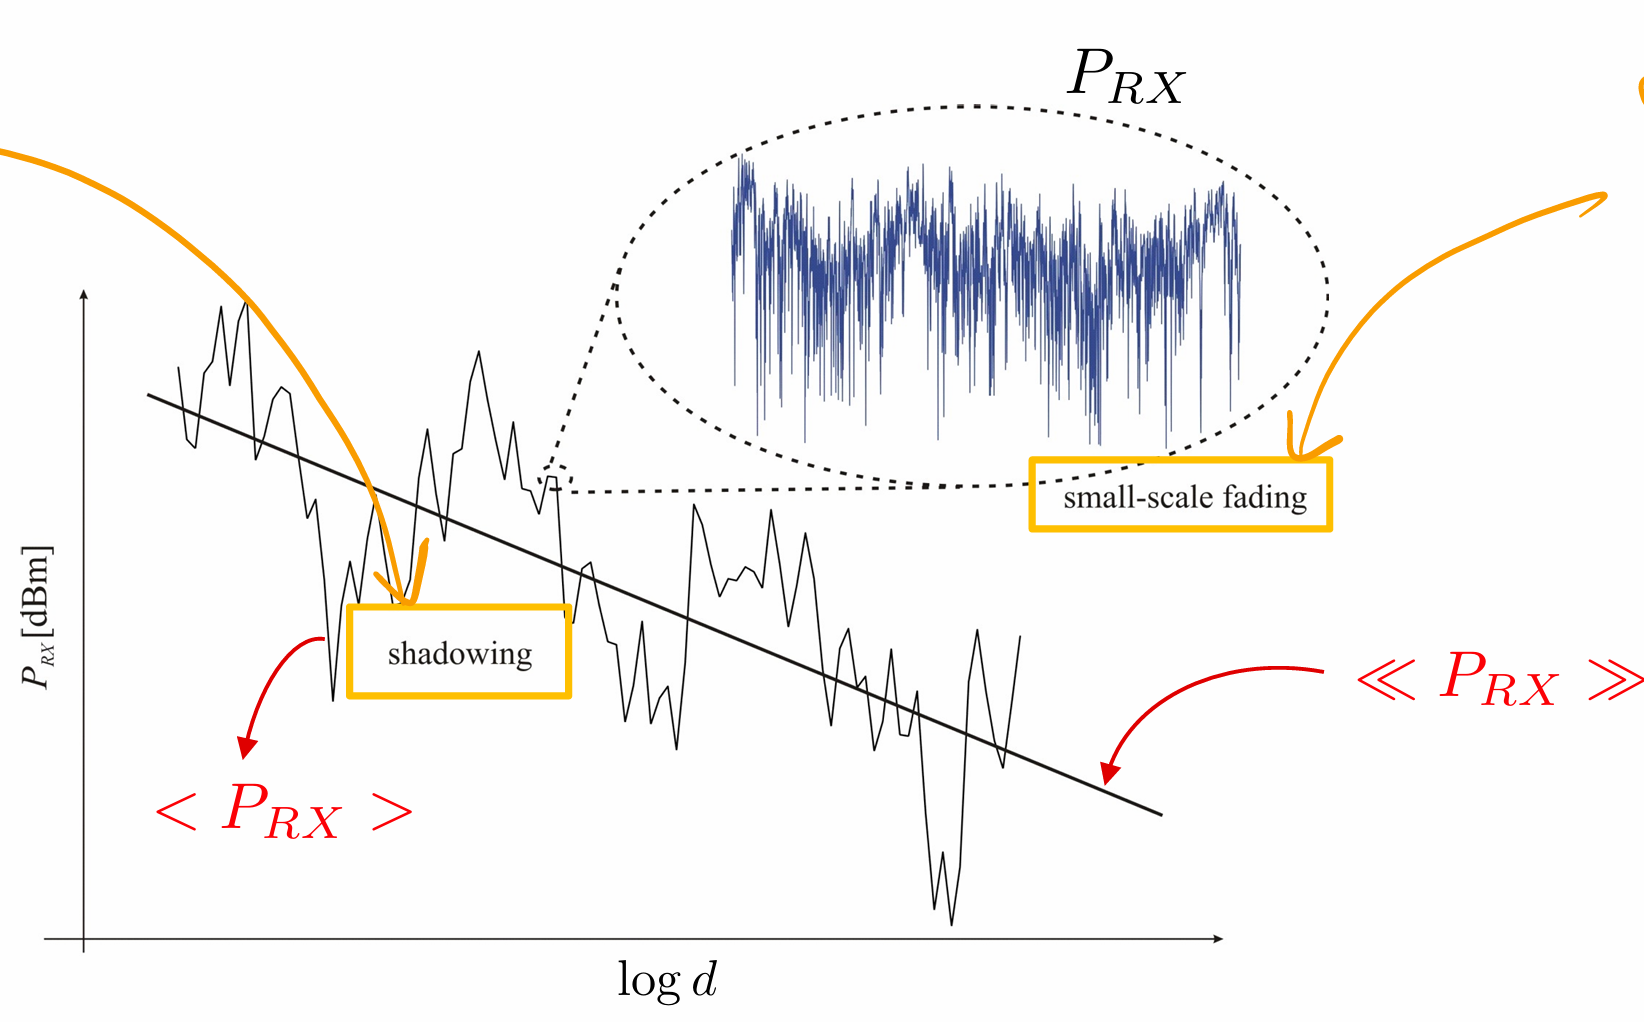
\includegraphics[width=0.8\linewidth]{"pictures/power-components.png"}
			\caption{Illustration of path loss, shadowing, and small-scale fading.}
		\end{figure}
	\end{frame}
	
	\section{Component 1: Path Loss Canonical Models}
	
	\begin{frame}{Defining the Large-Scale Trend}
		\begin{itemize}
			\item Path loss describes the average attenuation of signal power as a function of the distance $d$ between the transmitter and receiver.
			\item It represents the mean received power, denoted as $\ll P_{RX} \gg$.
			\item \textbf{Hypothesis}: We assume that the environment's large-scale properties are statistically homogeneous.
			\item This allows us to use a simple, empirically-validated mathematical form known as the \textbf{canonical path loss model}.
		\end{itemize}
	\end{frame}
	
	\begin{frame}{The Canonical Model Formulation}
		\begin{itemize}
			\item The model states that the average received power in dBm decays linearly with the logarithm of the distance.
			\[ \ll P_{RX}(d)\gg[\text{dBm}] = \ll P_{RX}(d_{0})\gg[\text{dBm}] - 10n \log_{10}\left(\frac{d}{d_0}\right) \]
		\end{itemize}
	\end{frame}
	
	\begin{frame}{The Canonical Model Formulation}
		\begin{itemize}
			\item Key Parameters:
			\begin{itemize}
				\item $d_0$: A reference distance, chosen in the far-field of the antenna.
				\item $n$: The \textbf{path loss exponent}, which characterizes the environment.
			\end{itemize}
			\item In terms of path loss $L(d) = P_{TX} - \ll P_{RX}(d) \gg$:
			\[ L(d)[\text{dB}] = L(d_0)[\text{dB}] + 10n \log_{10}\left(\frac{d}{d_0}\right) \]
		\end{itemize}
	\end{frame}
	
	\begin{frame}{Physical Origin of the Path Loss Exponent}
		\begin{itemize}
			\item The value of $n$ is determined by the dominant propagation mechanism.
			\item \textbf{Free Space ($n=2$)}: Derived from the Friis formula, where power density decreases with the surface area of a sphere ($1/d^2$).
			\[ P_{RX}(d) = P_{TX} G_{TX} G_{RX} \left(\frac{\lambda}{4\pi d}\right)^2 \implies \ll P_{RX} \gg \propto d^{-2} \]
		\end{itemize}
	\end{frame}
	
	\begin{frame}{Physical Origin of the Path Loss Exponent}
		\begin{itemize}
			\item \textbf{Over-the-Ground ($n=4$)}: At large distances in the two-ray model, destructive interference between the direct and ground-reflected paths leads to a much faster power decay.
			\[ P_{RX}(d) \approx P_{TX} G_{TX} G_{RX} \frac{h_{TX}^2 h_{RX}^2}{d^4} \implies \ll P_{RX} \gg \propto d^{-4} \]
			\item Other environments (urban, indoor) have values of $n$ between 2 and 6, determined empirically or through complex physical models.
		\end{itemize}
	\end{frame}
	
	\section{Component 2: Shadowing Statistical Model}
	
	\begin{frame}{Modeling Medium-Scale Variations}
		\begin{itemize}
			\item The path loss model gives the average power over all possible locations at a distance $d$.
			\item In reality, large obstacles like buildings or hills cause the \textit{local} average power, $<P_{RX}>$, to deviate from this global average. This is \textbf{shadowing} or slow fading.
			\item \textbf{Hypothesis}: The shadowing effect is a random process.
			\item \textbf{Observation}: Numerous measurement campaigns have shown that the variations of $<P_{RX}>$ in dB follow a \textbf{Normal (Gaussian) distribution}.
		\end{itemize}
	\end{frame}
	
	\begin{frame}{The Log-Normal Model}
		\begin{itemize}
			\item The local average received power is modeled as the mean power from the path loss model plus a random variable.
			\[ <P_{RX}>(d)[\text{dBm}] = \ll P_{RX} \gg[\text{dBm}] - L_{\sigma_L} \]
			\item $L_{\sigma_L}$ is a zero-mean Gaussian random variable with standard deviation $\sigma_L$.
			\[ L_{\sigma_L} \sim \mathcal{N}(0, \sigma_L^2) \]
		\end{itemize}
	\end{frame}
	
	\begin{frame}{The Log-Normal Model}
		\begin{itemize}
			\item The parameter $\sigma_L$ is the \textbf{shadowing variability} (in dB), which depends on the environment's clutter (e.g., 4 dB for open areas, up to 10 dB for dense urban).
			\item Since the power in dB is Gaussian, the power in linear units (Watts) follows a \textbf{log-normal distribution}.
		\end{itemize}
	\end{frame}
	
	\section{Component 3: Small-Scale Fading Models}
	
	\begin{frame}{Modeling Small-Scale Variations}
		\begin{itemize}
			\item Even within a small "local area" where $<P_{RX}>$ is constant, the instantaneous power $P_{RX}$ fluctuates rapidly as the receiver moves over distances of about half a wavelength.
			\item This \textbf{small-scale fading} is caused by the constructive and destructive interference of multiple signal copies (Multipath Components or MPCs) arriving from different directions.
		\end{itemize}
	\end{frame}
	
	\begin{frame}{Modeling Small-Scale Variations}
		\begin{itemize}
			\item The narrowband channel is modeled by a single complex coefficient $h(t)$:
			\[ y(t) = h(t) x(t) \]
			\[ h(t) = \sum_{n=1}^{N} a_n e^{j\Phi_n(t)} \]
			where $a_n$ and $\Phi_n(t)$ are the amplitude and phase of the $n$-th MPC.
		\end{itemize}
	\end{frame}
	
	\begin{frame}{The Rayleigh Fading Model (NLOS)}
		\begin{itemize}
			\item \textbf{Hypothesis}:
			\begin{itemize}
				\item There is a large number of MPCs ($N \to \infty$).
				\item There is no dominant (Line-of-Sight) path; all MPCs have comparable amplitudes.
				\item The phases of the MPCs, $\Phi_n$, are independent and uniformly distributed in $[0, 2\pi)$.
			\end{itemize}
		\end{itemize}
	\end{frame}
	
	\begin{frame}{The Rayleigh Fading Model (NLOS)}
		\begin{itemize}
			\item \textbf{Derivation}: By the Central Limit Theorem, the channel coefficient $h(t) = X(t) + jY(t)$ becomes a zero-mean complex Gaussian random variable.
			\item The envelope $|h(t)| = \sqrt{X^2 + Y^2}$ follows a \textbf{Rayleigh distribution}.
			\[ p(|h|) = \frac{|h|}{\sigma^2} \exp\left(-\frac{|h|^2}{2\sigma^2}\right) \]
			where $2\sigma^2 = \mathbb{E}[|h|^2]$ is the average power of the channel, which is given by the local average power $<P_{RX}>$.
		\end{itemize}
	\end{frame}
	
	\begin{frame}{The Rician Fading Model (LOS)}
		\begin{itemize}
			\item \textbf{Hypothesis}:
			\begin{itemize}
				\item There is one dominant, stable (LOS) component, plus a large number of weaker, scattered components.
			\end{itemize}
			\[ h(t) = \underbrace{A e^{j\theta}}_{\text{Dominant}} + \underbrace{\sum_{n=1}^{N} a_n e^{j\Phi_n}}_{\text{Scattered}} \]
		\end{itemize}
	\end{frame}
	
	\begin{frame}{The Rician Fading Model (LOS)}
		\begin{itemize}
			\item \textbf{Derivation}: The channel coefficient $h(t)$ is now a complex Gaussian variable with a \textbf{non-zero mean}.
			\item The envelope $|h(t)|$ follows a \textbf{Rician distribution}.
			\[ p(|h|) = \frac{|h|}{\sigma^2} \exp\left(-\frac{|h|^2 + A^2}{2\sigma^2}\right) I_0\left(\frac{|h|A}{\sigma^2}\right) \]
			\item This distribution is characterized by the \textbf{Rician K-factor}, the ratio of dominant to scattered power:
			\[ K = \frac{A^2}{2\sigma^2} \]
			\item As $K \to 0$, the Rician distribution converges to the Rayleigh distribution.
		\end{itemize}
	\end{frame}
	
	\section{Synthesis: Building the Complete Model}
	
	\begin{frame}{Step-by-Step Construction}
		\begin{itemize}
			\item We can now synthesize the complete model shown in Figure 4.8 by combining the three components sequentially.
			\item \textbf{Goal}: Generate a realistic series of received power values $P_{RX}(d)$ as a function of distance $d$.
		\end{itemize}
		\begin{block}{Procedure}
			\begin{enumerate}
				\item Define the large-scale trend with a path loss model.
				\item Add medium-scale variations by introducing shadowing.
				\item Superimpose small-scale fluctuations using a fading model.
			\end{enumerate}
		\end{block}
	\end{frame}
	
	\begin{frame}{Step 1: Path Loss Foundation}
		\begin{itemize}
			\item First, we calculate the mean received power $\ll P_{RX} \gg$ over the entire distance range using a canonical model.
			\item We choose an environment, which defines the path loss exponent $n$. For example, an urban micro-cell with $n=3.5$.
			\item We compute the mean power at a reference distance $d_0$.
			\[ \ll P_{RX}(d)\gg[\text{dBm}] = \ll P_{RX}(d_{0})\gg - 10n \log_{10}\left(\frac{d}{d_0}\right) \]
			\item This gives us the straight line (on a log-log plot) that represents the large-scale average.
		\end{itemize}
	\end{frame}
	
	\begin{frame}{Step 1: Path Loss Foundation}
		\begin{figure}
			\centering
			% Placeholder for the path loss line from Fig 4.8
			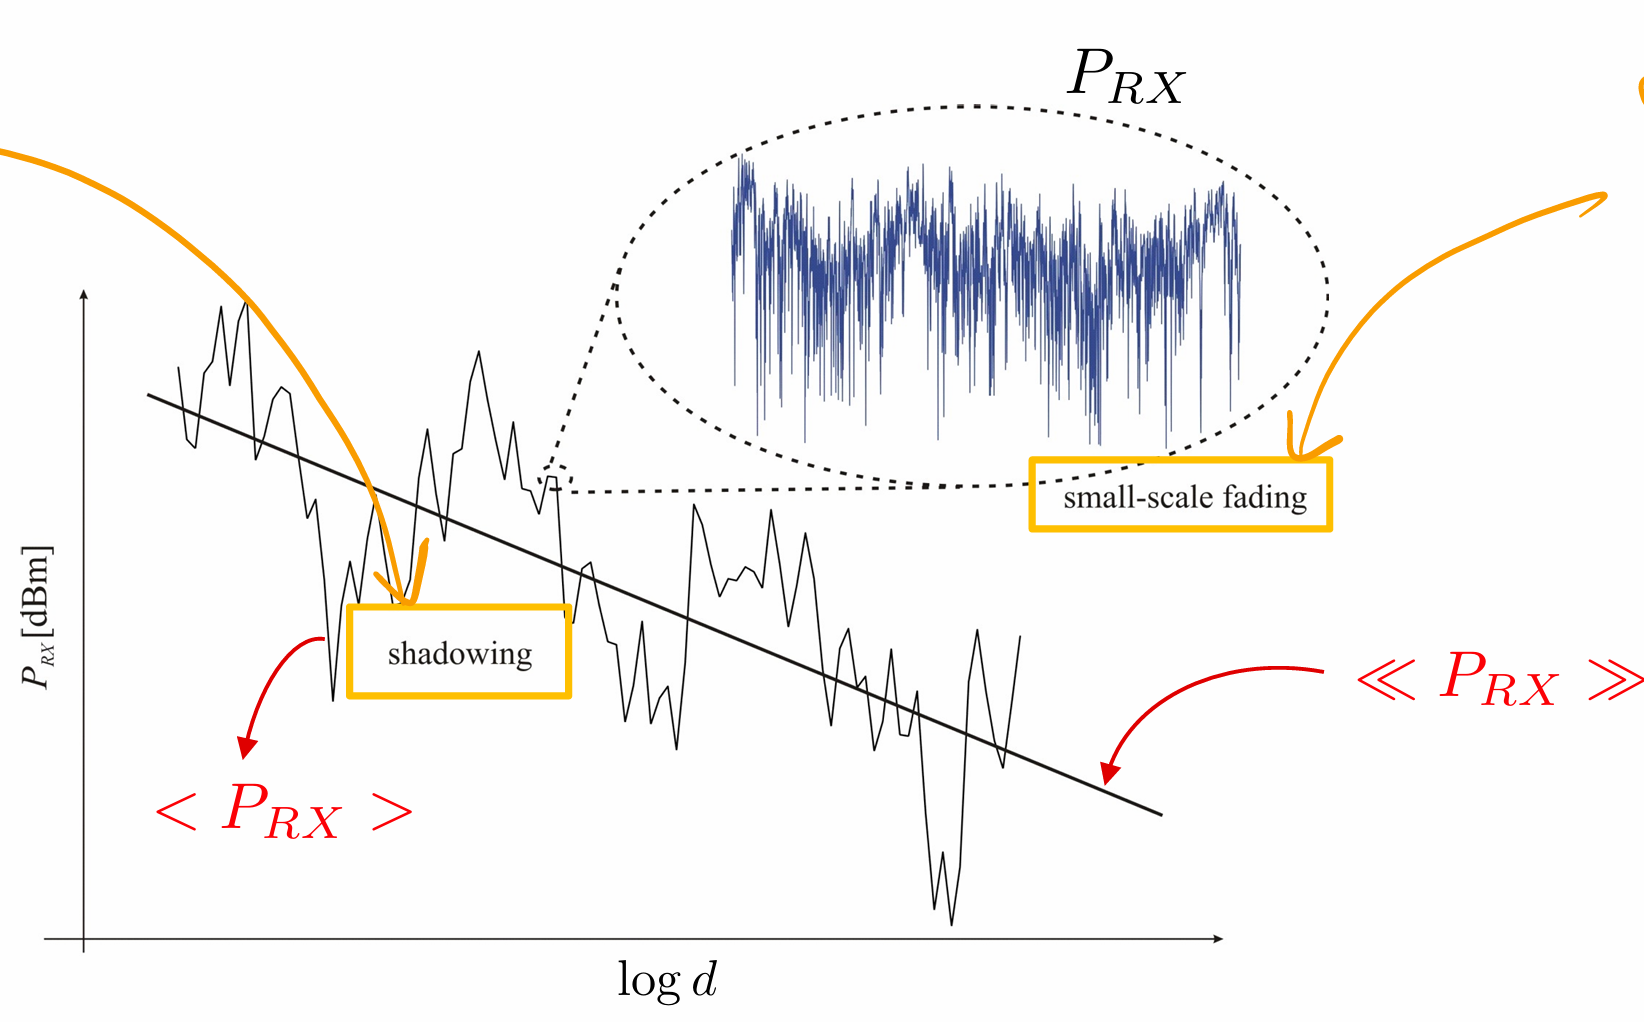
\includegraphics[width=0.7\linewidth]{"pictures/power-components.png"}
			\caption{The path loss model provides the mean trend line.}
		\end{figure}
	\end{frame}
	
	\begin{frame}{Step 2: Adding Shadowing}
		\begin{itemize}
			\item Next, we generate the local average power $<P_{RX}>$ by adding shadowing.
			\item We choose a shadowing variability $\sigma_L$ appropriate for the environment (e.g., $\sigma_L = 8$ dB for urban).
			\item For each point (or local area) along the path, we draw a random number from a zero-mean Gaussian distribution $\mathcal{N}(0, \sigma_L^2)$ and subtract it from the path loss mean.
			\[ <P_{RX}>(d)[\text{dBm}] = \ll P_{RX}(d)\gg[\text{dBm}] - L_{\sigma_L} \]
			\item This creates the slowly varying signal that "rides" on top of the path loss trend.
		\end{itemize}
	\end{frame}
	
	\begin{frame}{Step 2: Adding Shadowing}
		\begin{figure}
			\centering
			% Placeholder for the path loss + shadowing curve from Fig 4.8
			\includegraphics[width=0.7\linewidth]{"pictures/synthesis-step2.png"}
			\caption{Adding a log-normal random variable creates the shadowing effect.}
		\end{figure}
	\end{frame}
	
	\begin{frame}{Step 3: Superimposing Small-Scale Fading}
		\begin{itemize}
			\item Finally, we generate the instantaneous received power $P_{RX}$ by adding small-scale fading.
			\item At each point, the local average power $<P_{RX}>$ defines the average power of the fading distribution.
			\[ \mathbb{E}[|h|^2] \propto <P_{RX}>[\text{Watts}] \]
			\item We draw a random variable $|h|$ from either a Rayleigh (for NLOS) or Rician (for LOS) distribution, scaled by $<P_{RX}>$.
			\item The instantaneous power is then $P_{RX} = |h|^2 P_{TX}$.
			\item This process creates the rapid fluctuations that are characteristic of multipath interference.
		\end{itemize}
	\end{frame}
	
	\begin{frame}{Step 3: Superimposing Small-Scale Fading}
		\begin{figure}
			\centering
			% Placeholder for the final, complete curve from Fig 4.8
			\includegraphics[width=0.7\linewidth]{"pictures/synthesis-step3.png"}
			\caption{Superimposing Rayleigh/Rician fading on the shadowing curve yields the final model.}
		\end{figure}
	\end{frame}
	
	\section{Conclusion}
	
	\begin{frame}{Conclusion}
		\begin{alertblock}{A Unified Statistical Model}
			The total received signal power is a composite of three distinct statistical processes, each modeling a different physical scale of interaction:
			\begin{itemize}
				\item \textbf{Path Loss ($L(d)$)}: A deterministic function of distance, setting the mean power level.
				\item \textbf{Shadowing ($L_{\sigma_L}$)}: A log-normal (Gaussian in dB) random process modeling large-scale blockages.
				\item \textbf{Small-Scale Fading ($|h|^2$)}: A Rayleigh or Rician random process modeling multipath interference.
			\end{itemize}
		\end{alertblock}
	\end{frame}
	
	\begin{frame}{Conclusion}
		\begin{alertblock}{A Unified Statistical Model}[0.8\textwidth]
			By systematically combining these three layers—starting with the path loss trend, adding log-normal shadowing, and finally superimposing Rayleigh/Rician fading—we can construct a comprehensive and statistically accurate model of a wireless channel. This synthesized model is fundamental for simulating and predicting the performance of any real-world communication system.
		\end{alertblock}
	\end{frame}
	
	\section{Thank You}
	
\end{document}
